
%% bare_adv.tex
%% V1.4b
%% 2015/08/26
%% by Michael Shell
%% See:
%% http://www.michaelshell.org/
%% for current contact information.
%%
%% This is a skeleton file demonstrating the advanced use of IEEEtran.cls
%% (requires IEEEtran.cls version 1.8b or later) with an IEEE Computer
%% Society journal paper.
%%
%% Support sites:
%% http://www.michaelshell.org/tex/ieeetran/
%% http://www.ctan.org/pkg/ieeetran
%% and


%
\documentclass[10pt,conference,letterpaper]{IEEEtran}


\usepackage{cite}
\usepackage[pdftex]{graphicx}
\usepackage{amsmath}
\usepackage{algorithmic}
\usepackage{array}
\usepackage[caption=false,font=footnotesize]{subfig}
\usepackage{url}
\usepackage{caption}%add thi sentence can centering the caption.
\usepackage{multirow}% creat multirow table need to the packet
\usepackage{booktabs}% three table creating need to the packet
\usepackage{amssymb }% insert cuntermark
\usepackage{indentfirst}%��1.5���ַ�
\usepackage{ragged2e}
%\usepackage{mathtools}
\usepackage{amsmath}

\hyphenation{op-tical net-works semi-conduc-tor}
\makeatletter
\newcommand{\rmnum}[1]{\romannumeral #1}
\newcommand{\Rmnum}[1]{\expandafter\@slowromancap\romannumeral #1@}
\usepackage{bm}
\makeatother

\begin{document}
%
% paper title
% Titles are generally capitalized except for words such as a, an, and, as,
% at, but, by, for, in, nor, of, on, or, the, to and up, which are usually
% not capitalized unless they are the first or last word of the title.
% Linebreaks \\ can be used within to get better formatting as desired.
% Do not put math or special symbols in the title.
\title{A Survey on Motion Detecting Techniques and Influence Using WiFi Signals}

\maketitle

%\author{Lei~Wang,~\IEEEmembership{Member,~IEEE,}
     %   Linlin~Guo, Jialin Liu and ~Wei~Zhou}
%\renewcommand{\raggedright}{\leftskip=0pt \rightskip=0pt plus 0cm}
%\IEEEtitleabstractindextext{%
\begin{abstract}
%\raggedright
Some applications using WiFi signals have been increasing attention and studied for the past 2 decades such as Indoor location, human activity recognition, health monitoring and access control. According to the characteristic of WiFi signal, it is sensitive to the environment change. Development of those applications encounter challenges which contain indoor environment change, device diversity and motion influence. This article mainly addresses the problem of motion influence reflected by WiFi signals. Due to the fact that there are different affections on WiFi signal based applications. We survey influence of motion from these applications and deeply research developmental trend of WiFi signals. Specifically, we first show information of WiFi signals including Received Signal Strength (RSS), Channel State Information (CSI),  Arrive-of-Angle (AOA) and Time-of-Flight (TOF). Next, we summary challenges and problems which WiFi signals based applications are facing. Moreover, we show how to deal with the influence of motion in wireless network for these applications. We show that solutions correspond to the above mentioned problems in order to improve the accuracy of these application. Finally, we discuss that pay closed attention to opportunities and future research directions in this new and largely open area.
\end{abstract}

\IEEEpeerreviewmaketitle

\section{Introduction}

\subsection{Research Background and Significance}
During the past decade, there has been an exceptional development of wireless network and mobile device. WiFi signals are typically information carriers between a transmitter and a receiver. WiFi signals can also extend our senses, enabling us to see moving objects through walls and behind closed doors. The same thinking applies to security surveillance and saving hostages in current wireless network world. Of course, we also can recognize fine-grained gesture activity made behind a wall, such as push, pull and so on. The common application of WiFi signals is indoor location.

Location is playing an ever increasing role in mobile computing. Many of the most popular applications and services used today build on knowing the user's current location. For many of these applications, the accuracy of current technologies is adequate. However, we believe the next generation of mobile applications and services will need to a next generation location technology that provide accurate, reliable location information for indoor environments. We discussed how it has been designed and developed to provide application and service developers easy access to indoor location information. More broadly, we believe efficient and accurate room level location can open many new application opportunities.

In the static environment, motion influence come from two factor that environment changes and human motion; self-motion of objector has a important role in the influence of motion. In generally, some works neglect this factor due to this influence of self-motion was treated as least factor. However, according to experiment we show that self-motion influence has an important effective on micro-motion detection in some proposes works.

 Providing accurate and opportune information on people's location, human activities and behaviors is one of the most important tasks in pervasive computing. With the development and popularization of WiFi, surfing on Internet with mobile devices has become an indispensable of people's daily life. Human body is a strong electromagnetic energy absorption object, which may cause directional shadowing effect to wireless signal. Therefore, when the same device is placed at different position near human body, e.g. Shirt pocket or back pocket, the Received Signal Strength (RSS) measurement will be obviously deviated \cite{48,58}. Activity recognition means that leverage PHY layer information to indicate the human activities in indoor environment and then learn the specific pattern related with a specific human activity \cite{14}\cite{17}.


WiFi signals are typically information carriers between a transmitter and a receiver. The important work, see through walls with Wi-Fi, has been proposed by Fadel Adib from the MIT. WiVi \cite{61} show that WiFi can also extend our senses, enabling us to see moving objects through walls and behind closed doors. For example, we can identify the number of people in a closed room and their relative locations. We can also identify simples gestures made behind a wall. Further, by combining a sequence of gestures, a human can communicate messages to a wireless receiver without carrying any transmitting device. how one can use MIMO interference nulling to eliminate reflections off static objects and focus the receiver on a moving target. Second, how on can track a human by treating the motion of a human body as an antenna array and tracking the resulting RF beam. Further, Fadel Adib \cite{69} proposed a interest idea which captures the human figure through wall by using WiFi signals.

\textbf{How to differ reflection off objects from moving human} iterative nulling, which allows us to eliminate residual flash and the weaker reflections from static objects behind the wall.

\textbf{How does WiVi tracking moving objects without an antenna array?} To address this challenge, we borrow a technique called inverse synthetic aperture radar (ISAR), which has been used for mapping the surfaces of the Earth and other planets. ISAR uses the movement of the target to emulate an antenna array as shown in Figure~\ref{fig_antennaarray}.

\textbf{Indoor Location}: Indoor location applications\cite{5,12,13,19,20,21,22,23,24,26,27,
28,29,35,49,54,55,56,70,72,73,74,75} are common in our daily. Indoor location systems as mentioned in this paper are WiFi signals based, and others (Camera-based, Wearable sensors-based and so on) do not make the introduction. Motivated by demand of social life, indoor location systems\cite{13,19,20,22,23,24,26} which cater to different needs were proposed in recent years. According to the development history of study on indoor location, the goal of study mainly seeks to low hardware cost, high precision and deployment convenience. In order to decrease hardware cost, recent works \cite{19,20,22,23,28} leverages crowdsourced-based method to collect data. A few works \cite{23,26,35,49} leverage fine-grained CSI (PHY layer information) and mobility behavior to achieve high precision. The deployment convenience of indoor localization has play a important role in complexity indoor environment. There are recent works \cite{70,72,73,74,75,59} to adapt to dynamic environment such as multiple objects, dynamic target speed and reset furniture. D.Xuan team proposed some works \cite{54,55,56} which combined visual signal with electronic signal to obtain high precision and deployment convenience. In WiFi signals based study, this thinking is worthy of consideration.

\textbf{Human Activity Recognition}: Human activity recognition \cite{2,6,9,10,11,14,,45,46,47}
was widely used in Human-Computer Interaction (HCI),Senior health, hostage solution, security surveillance. Human activity recognition contains human activity, gestures and keyword recognition in practical public places. A few works \cite{2,11,15,16,43,44} proposed methods of coarse-grained activity recognition such as shopper's behavior \cite{11}, location-based activity recognition \cite{16}. On the basis of coarse-grained activity, gesture recognition \cite{42,45,46,47,62} get a attention in wireless application. WiSee \cite{46} leverages CSI to identify 9 gestures with an average accuracy of 94$\%$. WiGest \cite{47} leverages gesture recognition to control media player application actions with 96$\%$. The essence of keyword recognition \cite{63,64,66} is a fine-grained activity recognition: identify WiFi signals changes reflected by keystroke to get keyword according to different keywords correspond to different WiFi signals change.

\textbf{Access Control and User Authentication}: Access control and user authentication bring a new wave of research in room-area networks \cite{3}. Room-Area Networks (RAN) means range of wireless signal coverage. At present, recent works \cite{41,3,4,6,7,18,60} leverage users'locations to limit WiFi access and other services. CLAC \cite{4} proposed a design method which can detect user in indoor or outdoor by RSS and CSI. User authentication is an important part of access control \cite{31,32,36,39}. Legal user only has grant to access special service or resource in the current network environment, such as large company.

\textbf{Detecting Mobility}: Mobility information \cite{37}, as a new dimension information in addition to wireless signals, can benefit localization in a number of ways, since location and mobility are nature related in the physical world. Detecting mobility of target leverages WiFi signals change reflected by target motion \cite{1,10,68,71}. Speed and orientation are two properties of motion. A few works mainly resolve dynamic speed motion \cite{70,71}. High speed motion enhance change rate of WiFi signals in dynamic environment \cite{71}. On the basis of detecting mobility, motion tracking \cite{50,51,52,53,57} has developed in recent years.

\begin{figure}[hbt]
\centering
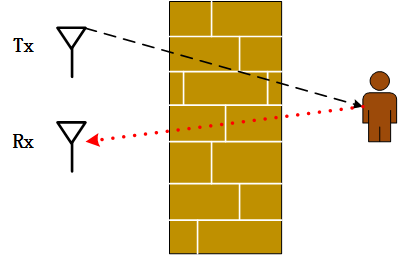
\includegraphics[width=2.0in]{fig/throughwall.png}
\caption{See Through Wall Using WiFi Signals}
\label{fig_throughwall}
\end{figure}

%\hfill mds

%\hfill August 26, 2015


\subsection{Challenges and Issues}

\textbf{LoS and NLoS}: According to the NLOS/LOS conditions, PHY layer setting

In general, Noise often are classified as following three part:
1) The first type of noise is the slight RSS fluctuation due to environment Gaussian noise.
2) The second type of noise is caused by small environment changes such as device perturbation in one's hand or people walking nearby.
3) Exists some impulsive noise in the RSS sequence for some type of mobile phones \cite{8}\cite{84}.

\subsection{Thesis Organization}
In this article, we survey this new trend of mobility enhancing human computing using WiFi signals. Specifically, we first study how to WiFi signals measures: what types of WiFi measures we can use and what types of mobility information we can acquire. Next, we discuss how mobility influent WiFi signals on different application in wireless networks. By introducing some application of WiFi signals, acquire the accuracy influence of motion in wireless networks. mobility offer enhancing localization accuracy, decreasing deployment cost and enriching location context.
Combining existing work and our own working experiences, we emphasize the principles and conduct a comparative study of the mainstream technologies. Finally, we conclude this survey by addressing future research directions and opportunities in this new and largely open area.
%\begin{itemize}

%\item To the best of our knowledge, this is survey about mobility influence of practical application based on WiFi signals(this is survey on application based on WiFi signals from the mobility influence). The above mentioned application based on WiFi signals contain indoor localization, human activity, target tracking and access control in wireless network.

%\item We list the different mobility patterns of those application and the corresponding challenges, as well as provide a comprehensive comparison for each category application in the term of accuracy, metric, device and cost.

%\item We provide that new solutions for the above mention challenge.

%\item Finally, we discuss the open research issues.

%\end{itemize}

\section{Motion types and Measuring Principles}
\subsection{Introduction of Related Technical Method}

\begin{figure}[hbt]
\centering
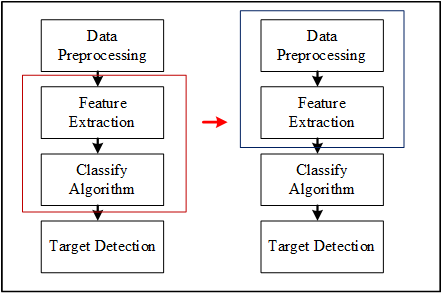
\includegraphics[width=2.5in]{fig/framework.png}
\caption{Framework of Design Systems}
\label{fig_framework}
\end{figure}

\textbf{Probability Model based}: Probability model based methods occurred in the previous work. Probability model construct by training collected information. However, probability model based method is not pervasive for different environment. this model has not invalidation when environment occurs change \cite{27}. Radio-map based techniques can be categorize into two broad categories: deterministic techniques and probabilistic techniques. Deterministic techniques represent the signal strength of an access point at a location by a scalar value, for example, the mean value, and use non-probabilistic approaches to estimate the user location. On the other hand, probabilistic techniques store information about signal strength distributions from the access point in the radio map and use probabilistic techniques to estimate the user location.

\textbf{Fingerprint based }: In indoor environment, fingerprint based methods, first collect fingerprint of WiFi signals in advance at known locations inside a building, and then identify the user��s location by matching the fingerprint of this user with the fingerprint stored in database. WiFi fingerprint-based schemes can provide meter-level indoor localization accuracy at the expense of explicit site-survey (its high deployment cost and low adaptiveness to environment change hinders the practical effectiveness) \cite{74}.

1) Among these approaches, a hot research trend is to incorporate crowd-souring model and built-in sensors in today��s smart-phone.

2) We believe there are plenty of room for improving the localization accuracy while reducing or even eliminating the dependence of site-survey and noisy inertial sensors.

3) It has been widely known that the RSS value is affected by many factors, e.g., the RSS values collected at the same location using same devices with same WiFi APs could fluctuate to a few db depending on how users hold and block the signal

\textbf{Crowdsourcing based}: Crowdsourcing based method leverages large mobile devices which are spread over users to collect data information from existing surround environment. It reduce cost of people, financial resources by using crowdsourced. However, crowdosourcing based method has some challenges in the practical environment. First, Data information collected by crowdsouring is not sure safety and high quality due to identify of mobile device is stranger. Second, location distribution of collecting information is uneven. If so that, Collecting information can not represent global state of indoor environment. Third, diversity of different mobile device bring small difference to enhanced the inaccuracy data information \cite{22}. In summary, Goal of Crowdsourcing based get high accuracy and low computational requirements.



\subsection{Motion Types}
In general, WiFi signals are sensitive to indoor environment changes which contain different influence from different motion type in the indoor environment. It is common hard questions for most researchers to proposed a effective methods adapting dynamic complexity environment. Of course, this questions are challenges. In every research work, authors often show that exists challenges and hard in their work. Motion influence play a important role in wireless network. Goal of this paper mains analysis influence of mobility  for WiFi signal, and try to find a adaptive solutions which estimate mobility influence in different scenarios using fit metric. If so that, mobility factor treat as addition dimension to improving WiFi signal sensing accuracy in complexity indoor environment.

Motion types dived into three classes. The first, target mobility has important influence on WiFi signal is common phenomenon in practical daily life for people. For example, target often walks in public place. Second, surround object mobility result in WiFi signals change to affect target identify. This part is most important challenge for current wireless environment application. For example, Indoor location systems in recent often face with non-target interference. It is hard to identify target and non-target using WiFi signals if target and non-target without attach devices stay static in indoor environment. Similar problems have occurred, non-target mobility have non-negligible influence to  localizing target. Specifically, CSI (Channel Static Information) has high sensitive to surround environment changes, even small change may product important influence. So, non-target mobility influence for WiFi signal is key point to solute high location problem.

\textbf{Target Mobility}: Target mobility need to face some challenges. Static target is not often occur in practical daily, moving state is common behavior due to human activity. So, we proposed some methods or systems to solute Target mobility such as detecting moving target or locating mobility target and so on. What dose occurs in target mobility? It can change distance of target from transmitter to receiver, enrich multi-path effect, add environment complexity. The classic method leverages LoS identify to locate target or detect moving target \cite{10}.
\begin{figure}[hbt]
\centering
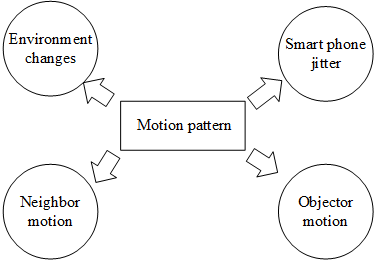
\includegraphics[width=2.0in]{fig/motion.png}
\caption{Motion Pattern}
\label{fig_motion}
\end{figure}
\begin{figure}[hbt]
\centering
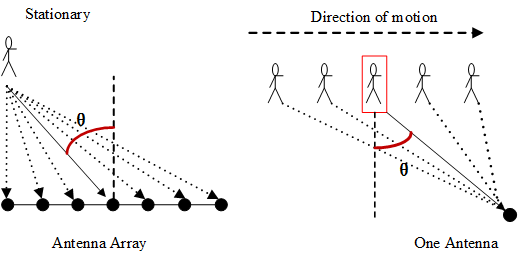
\includegraphics[width=3.0in]{fig/antennaarray.png}
\caption{A Moving Object as Antenna Array}
\label{fig_antennaarray}
\end{figure}
\begin{figure}[hbt]
\centering
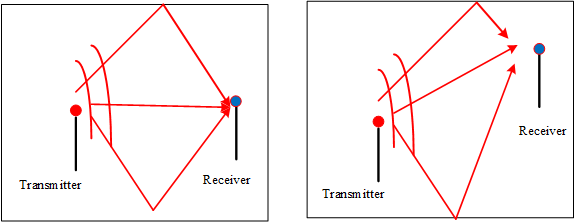
\includegraphics[width=3.0in]{fig/targetmove.png}
\caption{Change of the target moving}
\label{fig flow}
\end{figure}

\textbf{Non-target Mobility}: Non-target mobility means other move object which are normal daily in public workplace such as laboratory or office. Next, Non-target mobility bring a complexity computing of WiFi signals influence in wireless networks. Sometime, Non-target mobility reflected by WiFi signal more than high target. In this event, how to distinguish  mobility influence of target from non-target is essential and important for application which depend on WiFi signals change.

\textbf{Indoor Environment Changes}: Indoor environment changes contains several aspects in the practical environment. In this paper, we give a specially definition of indoor environment from two aspects. One is that add some things to indoor or remove some things. Second is that rearrange the furniture in the indoor. In simple speaking, we only explain simple cases in our daily. Indoor environment changes only impact the multi-path effect.

\textbf{Wireless Device Jitter}: Target with handhold mobile device is hard to keep balance state in motion scenarios. Mobile device jitter result from arm movement of target can cause  small changes of WiFi signal. Just so, this small change is hard different from change of WiFi signals from target self moving.

\subsection{Measuring Principals and Motion Informations}
\textbf{Equipment Requirement}: 1) The CSI tool is built on the Intel Wi-Fi Wireless Link 5300 802.11n MIMO radios \cite{40}, using custom modified firmware and open source Linux wireless drivers. The IWL5300 \cite{88} provide 802.11n channel state information in a format that reports the channel matrices for 30 subcarrier groups, which is about one group for every 2 subcarriers at 20HMz or one in 4 at 40HMz. 2) Atheros CSI Tool \cite{87} is open source 802.11n measurement and experimentation tool. It enables extraction of detailed PHY wireless communication information from the Atheros WiFi NICs, including the Channel State Information(CSI), the received packet payload, and other additional information such as the time stamp, the RSS of each antenna and the data rate. The differences between IWL5300 card and Atheros-CSI-Tool were showed as follows in Table~\ref{tab:CSI_Tool}.
%introducting CSI-Tool
\begin{table}[htbp]
\center
\scriptsize
\caption{\label{tab:CSI_Tool}CSI Tool}
\begin{tabular}{ccccc}
\toprule
 Types & Subcarriers& Frequency & Modified firmware & Year \\
\midrule
IWL5300 &30 & 20HMz or 40HMz& Y & 2011 \\
Atheros &56 &20HMz&N &2015 \\
Atheros &114& 40HMz&N &2015 \\
\bottomrule
\end{tabular}
\end{table}

\section{Performance and Metrics}
Wireless radio propagation in compact environment could be modeled as a superposition of large-scale path-loss, middle-scale shadowing, and small-scale multi-path fading \cite{48}. A wireless signal traverses in all radial directions, and reflects off walls, furniture, and other objects. Due to reflections, multiple copies of the same signal arrives at the receiver, each undergoing different delay and attenuation - a phenomena which is commonly called multi-path. Definition of the direct path is the straight line joining the transmitter and the receiver. A wireless signal is composed of a direct path, and other reflected components, and suffers attenuation as it propagates from the transmitter to the receiver. Indoors, wireless attenuation is mainly caused by path-loss, and multi-path reflections.

RADAR \cite{21} operates by recording and processing signal strength information at multiple base stations positioned to provide overlapping coverage in the area of interest. It combines empirical measurements with signals propagation modeling to determine user location and thereby enable location aware services and application.

Zee\cite{19} Notes that only mobility information in employed but no WiFi measurements are required during this trajectory embedding process. To eventually generate a fingerprint database, however, zee still expects users to record WiFi measurements during their moving paths, which will then be annotated with the locations estimated from trajectory embedding.
The main Information measurements of WiFi signals are summarized as follows:

\begin{itemize}
\item \textbf{RSS}

The wireless channel between the client and the AP is expected to vary under environmental or device mobility. This is because the fine-grained multi-path structure may change if there are moving objects in the environment, or the device itself moves. These fine-grained variations of the wireless channel can not be captured by RSS because it only captures an aggregate indicator of all the multi-path components.

It is possible to estimate a crude distance between the transmitter and the receiver by using the received energy at the receiver $(P_{R})$ in the path-loss equation:
\begin{equation}\label{1}
  P_{R}=P_{0}-10\gamma log{(d)}
\end{equation}
where $P_{0}$ is the received energy at a distance of 1m from the transmitter, $d$ is the distance between the transmitter, and the receiver in meters; and $\gamma$ is the path loss exponent. $\gamma$ depends on the propagation characteristics of the received signal. Earlier approaches have typically used RSS as the received energy $(P_{R})$ in the above path loss equation \cite{12}. However, RSS is an union of the energy of all the signal paths-direct as well as multi-path reflections. If we use RSS as $P_{R}$, we will need to estimate the propagation characteristics of all the signal paths, to correctly choose the path-loss exponent. Unfortunately, today's WiFi cards do not expose any specific multi-path information, making it difficult to model the aggregate signal(RSS), we show that it is easier to only use the energy of the reflected paths, it can be a robust indicator of distance, even in dynamic indoor environments.
\item \textbf{CSI}\\
CSI is not a simple extension of RSS on physical subcarrier but it reveals totally different information on frequency selective fading process. The CSI is reported as a matrix of complex numbers representing the channel gain for every subcarrier and for every transmit-receive antenna pair. By an appropriate Inverse Fast Transformation (IFFT), the frequency-domain CSI can be translated into the time-domain power-delay profile (PDP). PDP captures the energy of the different paths incident at increasing delays. Since, the direct path traverses the minimum distance amongst all the received paths, its energy will likely appear in the earliest component of the PDP.
\item \textbf{TOF}\\
Systems that use timestamps reported by WiFi cards can obtain Time of Flight (TOF) at a granularity of several nanoseconds, requiring in ranging error of few meters. The time it takes for its signal means to travel from its transmit antenna to the reflecting body, and then back to each of its receive antennas. WiTrack \cite{61} obtains an initial measurement of the TOF using FMCW transmission technique; it then cleans this estimate to eliminate multi-path effects and abrupt jumps due to noise.FMCW transmits a narrowband signal whose carrier frequency changes linearly with time. To identify the distance from a reflector, FMCW compares the carrier frequency of the reflected signal to that of the transmitted signal. Since the carrier frequency is changing linearly in time, delays in the reflected signals translate into frequency shifts in comparison to the transmitted wave.

Specifically, we know from basic electromagnetic that as a signal propagates in time, it accumulates a corresponding phase depending o its frequency. The higher the frequency of the signal, the faster the phase accumulates. To illustrate, let us consider a transmitter sending a signal to its receiver. Then we can write the wireless channel $h$ as :
\begin{equation}\label{5}
h=ae^{-j2\pi f\tau }
\end{equation}

where $a$ is the signal magnitude, $f$ is the frequency and $\tau$ is the TOF. The phase of this channel depends on TOF as:
\begin{equation}\label{6}
  \angle h=-2\pi f \tau mod 2\pi
\end{equation}
Notice that the above equation depends directly on the signal's TOF and hence, we can use it to measure the TOF $\tau$ as
\begin{equation}\label{7}
 \tau =-\frac{\angle h}{2\pi f} mod \frac{1}{f}
\end{equation}
The above equation gives us the TOF modulo $1/f$. Hence, for a WiFi frequency of 2.4GHz, we can only obtain the TOF modulo 0.4 nanoseconds.
\item \textbf{AOA}\\
In general, we leverage AOA information to locate target in indoor environment. how to get AOA information from wireless network by the smart phone or other mobile device. MUSIC algorithm can get AOA information. AOA means wireless signals of arrive of angle from transmitter to receiver. Moreover, AOA treat as add dimension information to locate target for improving accuracy of location. The key point need to get transmitter location information, then by MUSIC \cite{49} algorithm computing AOA information, next leverage triangle relation to locate target. AOA measures [-90,90] in antenna array.
A wireless transmission from the client arrives at several angles at the AP. If we can determine the angle of the direct path or ANDP. It is possible to combine the angle of the client with her distance, ultimately yielding her location. Existing AOA estimation algorithms analyze the received signal on multiple antennas to find out the angular components of the signal \cite{81}. The key idea is to analyze the phase of the received signal, a quantity which changes linearly by 2$\pi$ for every wavelength $(\lambda)$ traversed by the signal. For the simplicity of explanation, consider s single path between the transmitter and the receiver. Let us consider that the AP has only two antennas, placed at a distance of $\frac{\lambda}{2}$. Let $\theta$ be the angle at which the signal arrives at the two antennas. The signal travels an extra distance before reaching the second (left) antenna. This extra distance $(\Delta)$ can be approximated as:
\begin{equation}\label{2}
  \Delta d=\frac{\lambda }{2}sin(\theta )
\end{equation}

We know that an extra distance $\Delta d$ will result into a phase difference $(\Delta \phi)$:\\
\begin{equation}\label{3}
 \Delta \phi =\frac{2\pi \Delta d}{\lambda }
\end{equation}

Thus, by observing the phase difference$(\Delta \phi)$ of the arriving signal, we can find the angle-of-arrival as:\\
\begin{equation}\label{4}
  \theta =arcsin( \frac{\Delta \phi}{\pi})
\end{equation}

The above explanation assumes that the arriving signal has only one angular component. In reality, a wireless signal will propagate through multiple paths. AOA estimation algorithm can identify the angles of multiple paths by using many antennas.


With the proliferation of WiFi APs with multiple antennas to support MIMO communications, antenna array based techniques which use multiple antennas at the AP have gained interest recently. The basic idea of these systems is to calculate the AOAs of the multiple signals received at each AP, find the AOA of the direct path to the target, and then apply triangulation to localize \cite{20}\cite{12}\cite{76}\cite{78}\cite{79}.

\begin{table}[htbp]
\center
\scriptsize
\caption{\label{tab:test} Characteristics of WiFi Signals in Indoor Localization}
\begin{tabular}{cp{1cm}cp{1cm}p{1cm}}
\toprule
Information & Accuracy & Device & Adaptation & Complexity \\
\midrule
RSS& 2 m & Common Device  &  Low & Low\\
CSI& 1 m &5300 or Atheros or USRP & Middle & Middle\\
AOA& 1 m & Antennas  & High & Middle\\
TOF& 60 cm& Specific Device & High & High\\
\bottomrule
\end{tabular}
\end{table}

Different WiFi signals provide different accuracy in table 1. Accuracy of indoor location has most high accuracy using TOF, then AOA, RSS is the worst. But, RSS information for common device is feasible. Table 1 show that the accuracy means average accuracy in the above applications.

\begin{table}[htbp]
\center
\scriptsize
\caption{\label{tab:test}RF Attenuation in Common Building Materials at 2.4GHz \cite{80}}
\begin{tabular}{cc}
\toprule
 Building Materials & 2.4 GHz \\
\midrule
Glass & 3 dB \\
Solid Wood Door 1.75inches & 6 dB \\
Interior Hollow Wall 6 inches & 6 dB \\
Concrete Wall 18 inches & 18 dB\\
Reinforced Concrete & 40 dB\\
Brick 3.5 inches & 6 dB\\
Steel Fire and  Exit Door 2.5 inches& 19 dB\\

\bottomrule
\end{tabular}
\end{table}
%\begin{table}[htbp]
%\center
%%\scriptsize
%\caption{\label{tab:test}Devices based Indoor Localization}
%\begin{tabular}{lcl}
%\toprule
% System & Technologies & Accuracy \\
%\midrule
%Pinpoint & RF TOA & 1.3 m \\
%Cricket & TDOA(Ultrasound+RF) & 5 cm \\
% RADAR & WiFi RSS & 5.9 m \\
 %Horus & WiFi RSS & 2 m\\
% TIX & WiFi RSS & 5.4 m\\
 %Virtual Compass & WiFi RSS & 3.2 m\\
%\bottomrule
%\end{tabular}
%\end{table}

\end{itemize}
\begin{table}[htbp]
\center
\scriptsize
\caption{\label{tab:test}Summary of Application Using WiFi Signals}
\begin{tabular}{ccccc}
\toprule
 Citation & RSS & CSI & AOA & TOF \\
\midrule
RADAR\cite{21} & \checkmark & & &  \\
Horus\cite{27} & \checkmark &  & &  \\
Zee\cite{19} &  & \checkmark & &   \\
SpinLoc\cite{35} & & \checkmark & &  \\
CLAC\cite{4} & \checkmark & \checkmark & &  \\
Arraytrack\cite{76} & & & \checkmark &  \\
Ubicarse\cite{20} &  &  & \checkmark  &   \\
SpotFicite\cite{49} & & & \checkmark & \checkmark \\
Chronos\cite{5} & & & &\checkmark \\
\bottomrule
\end{tabular}
\end{table}

\begin{table}[htbp]
\center
\tiny
\caption{\label{tab:test}Activity Recognition Using WiFi signals}
\begin{tabular}{cp{1cm}cp{1cm}p{1cm}p{1cm}}
\toprule
Citation & Technical & Average Accuracy & Devices & AP Number & Classification \\
\midrule
Stephan Sigg & RSS & N/A & USRP & one or many & K-NN \\
WiSee  &Doppler Shifts & $94\%$ & USRP & many & N/A \\
WiGest  & RSS  & $87\%$ & CTOS & one or many & N/A \\
WiFall  & CSI & 87$\%$ & Intel 5300  & 1& SVM \\
E-eyes  & CSI& 92$\%$ & Intel 5300  & 1 & NPC \\
\bottomrule
\end{tabular}
\end{table}

%three-table is as follows.

% the second table

\begin{table}[htbp]
\center
\tiny% design size of font from the table
\caption{\label{tab:test}Comparison of Different RF-Based Passive Localization Systems \cite{xu2013scpl}}
\begin{tabular}{ccccc}
\toprule
  & Grid Array & RTI & NUZZER & SCPL \\
\midrule
Measured physical quantity & RSS variance & RSS attenuation & RSS change & RSS change \\
Non-LoS Localization & No & Yes & Yes & Yes \\
Nodes Density  & High & High & Low & Median  \\
Prior knowledge of node locations & Yes & Yes & No & No\\
Tracking static subjects & No & Yes & Yes & Yes \\
Deployment scale & Median & Small & Large & Large \\
Training Overhead & Low & Low & High & Median \\
\bottomrule
\end{tabular}
\end{table}

\textbf{Non-invasive Human Detect}: Wireless non-invasive human detection systems detect and localize humans via their impact on received signal, while targets carry no wireless-enabled devices.

\textbf{Device-free Passive Motion Detect}: The detected individual neither carrying any device nor actively participating in the detection progress.


%SpinLoc\cite{35}
On observing that the statistical spectral structures of small-scale multi-path signals possess resistance to irrelevant background dynamics while retaining sensitivity to nearby human locomotion. We propose to leverage the histogram feature of the subcarrier amplitudes as signatures for our omnidirectional passive human detection.

\textbf{A Number of Human Detect}: In order to address the non-linearity of the impact of multiple subjects, we propose a successive cancellation based algorithm to iteratively determine the number of subjects. SCPL \cite{xu2013scpl} models indoor human trajectories as a state transition process, exploit indoor human mobility constraints and integrate all information into a conditional random field (CFR) to simultaneously localize multiple subjects.

\textbf{Indoor Localization}: Indoor localization systems using WiFi infrastructure should ideally satisfy the following three requirements.
\begin{itemize}
\item \textbf{Deployable}: They should be easily deployable on existing commodity WiFi infrastructure without requiring any hardware of firmware changes at the access points (APs); they should only work with information like RSS and CSI that is already exposed by commodity, deployed APs.
\item \textbf{Universal}: They should b e able to localize any target device that has a commodity WiFi chip and nothing else. They should not require the target to have any other hardware, be it sensors such as accelerometers, gyroscopes, barometers, cameras, etc., or radios such as UWB, ultrasound, Bluetooth LE, etc.
\item \textbf{Accurate}: They should be accurate, ideally as accurate as the best known localization systems that use wireless signals (even including those that do not satisfy the above two requirements). To the best of our knowledge, the most accurate such localization systems are ArrayTrack \cite{76} and Ubicarse \cite{20} and these systems achieve an accuracy ranging from 30-50 cm in office environments. Achieving such accuracy would be the target.
\end{itemize}

\textbf{Detecting different motions}: The wireless channel between the client and the AP is expected to vary under environmental or device mobility. This is because the fine-grained multi-path structure may change if there are moving objects in the environment, or the device itself moves. These fine-grained variations of the wireless channel can not be captured by RSS because it only captures an aggregate indicator of all the multi-path components. On \cite{60} observing that the statistical spectral structures of small-scale multi-path signals possess resistance to irrelevant background dynamics while retaining sensitivity to nearby human locomotion. We propose to leverage the histogram feature of the subcarrier amplitudes as signatures for our omnidirectional passive human detection

\textbf{Tracking user behavior}: In the air user interfaces can be divide into two classes. The first class is based on defining a limited set of gestures and using machine learning to learn patterns and classify gestures into the learned categories. The second class includes interfaces enabled by systems such as RF-IDRAW \cite{51} and WiDraw \cite{52}. These interfaces require no priori learning and can track an arbitrary set of hand motions,enabling a much richer set of applications. Note that only mobility information in employed but no WiFi measurements are required during this trajectory embedding process. To eventually generate a fingerprint database, however, zee still expects users to record WiFi measurements during their moving paths, which will then be annotated with the locations estimated from trajectory embedding


\section{How to deal with Motion Influence}

\subsection{Advantage}

Some of previous works have been designed to avoid mobility behavior due to mobility can impact on the change of WiFi signals. We surveys a large amount of papers in recent years to study motion influence. There are four points are summarized as following.

\textbf{Enrich Multi-path Information}:
Multi-path contains different numbers of paths according to different indoor environment, a few paths tend to dominate as they suffer minimal attenuation. In general, there are 6-8 paths in common indoor environment. Understanding patterns of human indoor movement can be valuable in identifying hot spots and corridors that help energy management and commercial site selection. DeMan \cite{17} provides a non-intrusive and private solution to capturing indoor locations.

Multi-path effect are common exists in indoor environment in wireless network. Even it is not avoid for common workplace. Human move can reset floor plan of environment, multi-paths will change adaptively. some works have deeply study multi-path information to improving accuracy of indoor location. Of course, the most related work is that identify LOS and NLOS of multipath in indoor environment \cite{8}\cite{84}. LiFi \cite{8} mainly show that identify LOS by using skewed distribution of CSI. Moreover, Phaseu \cite{84} completes real-time LoS identify in indoor environment. Other works select several paths from multi-path to complete indoor location or human activity recognition \cite{18}. (Wireless-based device-free human sensing has raised increasing research interest and stimulated a range of novel location-based services and human-computer interaction applications for recreation, asset security and elderly care. A primary functionality of these applications is to first detect the presence of humans before extracting higher-level contexts such as physical coordinates, body gestures, or even daily activities.

In the presence of dense multi-path propagation, however, it is non-trivial to even reliably identify the presence of humans. The multi-path effect can invalidate simplified propagation models and distort received signal signatures, thus deteriorating detection rates and shrinking detection range. In this paper, we characterize the impact of human presence on wireless signals via ray-bouncing models, and propose a measurable metric on commodity WiFi infrastructure as a proxy for detection sensitivity.

This paper can harness multi-path for a higher detection rate and wider sensing range with standard WiFi devices instead of avoiding multi-path to tradeoff detection reliability with sensing coverage. They do an in-depth analysis on how human presence alters wireless signals under different propagation mechanisms, and demonstrate that (1) human-induced reflections potentially extend detection range; (2) multi-path superposition status can lead to varied detection sensitivity.

In summary, multi-path information is worthy to study and application. How to leverage multi-path information is a interest research topic for us.

%\textbf{Enhancing security of access control}

\textbf{Reducing Cost of Device}: WiVi proposed a moving object as antenna array(ISAR) \cite{61}. This method can reduce the cost of device, and improve performance of those application such as indoor location, human tracking and access control. WiVi leverages MIMO interference nulling to eliminate reflections off static objects and focus the receiver on a moving target. by human moving, WiVi can identify the number of people in a closed room and their relative locations. IF people do not move, we are unable to identify the number of people in a closed room.

\textbf{Improving Accuracy of Indoor Location}: SpinLoc \cite{35} make a 360 degree rotation at her current location. Using the signals recorded during the rotation, and the already-known AP location, SpinLoc computes the location of the user. At the same time, SpinLoc relies only on the signal strength of the direct signal path. PinLoc \cite{77} find evidence that channel responses from multiple OFDM subcarriers can be a promising location signature. In other words, motion information provides different view to estimate object location in complex indoor environment.

\textbf{Dropping the Dependence to Indoor Environment}: Wireless signals are sensitive to indoor environment. Signatures of WiFi signals certainly vary over time and environment. Unfortunately, this characteristic bring more challenge for WiFi based application. Fingerprint-based indoor location cannot common application due to signature will change with environment changes. Most authors have try to propose a pervasive method of indoor location to deal with dynamic environment problems.
\subsection{Disadvantage}
Anything have two aspect, one is good, other one is bad. Motion has not only bring few advantage points, but also takes  few several disadvantage points such as increasing the complication of indoor environment, reducing reliable information of WiFi signals and destroying quality of data sets. Taken as a whole, data pre-processing and feature detection are two difficulties in the whole framework of systems with mobility based on WiFi signals.

\textbf{Increasing the Complication of Indoor Environment}: We study few application systems on the common workplace within more people. People either keep static behavior or keep move behavior. Some of previous works often assume that have no move people, or treat move people as special noise. With the deep researches of WiFi-based applications, mobility influence for WiFi signals can not neglect in indoor environment. Different indoor environments have different mobility behaviors is a challenge, and lead to infeasible of previous technics in new indoor environment. Mobility behavior change multi-path and indoor arrangement. A person's mobility not only influence itself, but also affect other persons, even target.
WiGest\cite{47} showed that as long as the interfering user is more than 4ft away, it has no-effect on accuracy. However, a close-by user by less than 3ft reduces accuracy of the gesture recognition.

\textbf{Contaminating Data Sets of WiFi Signals}: Data sets are sensitive to indoor environment. In general, data sets of WiFi signals contain RSS and CSI collected in indoor environment. Mobility behavior has more important influence on WiFi signals than static behavior. It is difficult to distinguished target's data from collecting data sets without using special technique. Therefore, we collected data sets which contain target's data, mobility data and other noise data. For other noise data, researchers proposed few available methods to resolve them. However, mobility behavior has never a feasible method to resolve it. At present, researchers often reinforce data preprocess to get high quality data sets in wireless network application.

\textbf{Making the Preprocessing more Difficult}: Due to complication of mobility behavior, preprocess phase becomes more hard than previous phase without mobility behavior. Static behavior can cause a small change of WiFi signals, mobility behavior can cause a large change. Outlier occur lead to a problem which is hardly distinguished between outlier and mobility behavior. At the same way, difference between target mobility and non-target mobility is small. These problems mentioned above require high-efficient of pre-processing stage to achieve high accuracy.

\textbf{Increasing the Consumption of Hardware Cost}: Mobility behavior increases instability of data sets collected by mobile device, and reduces performance of WiFi-based systems. In order to get high accuracy, it need to increase APs (5-6) and other sensors (accelerator, gyroscope). At present, few works combine WiFi signals with sensor data information to achieve the goal which only dependent on WiFi signals without mobility behavior. In future researches, the trend which WiFi-based application systems develop reduces the demand of equipment, and gradually depend on fine-grained wireless information. As a result, reducing the consumption of hardware cost is challenge for our study.

\subsection{Solutions}
We firstly make a simple introduction about a few problems of mobility behavior before give solutions in this section. These problems are divided into two categories in broad terms. The first problem is that treat mobility behavior (mobility behavior means non-target mobility behavior, target still keep static behavior) as a part of indoor environment; the second problem is that distinguish between target mobility behavior and non-target mobility behavior.

\textbf{Problem 1}: Avoiding motion occur is the most simple method, However, it is difficulty and impossible for indoor environment such as public places, office and family. Therefore, how to deal with the influence of non-target mobility behavior for static target in wireless coverage of indoor environment?

\textbf{Solution 1}: In general, recent works leverage fingerprint-based method to match RSS and CSI collected by Receiver. but, there is a question which mobility behavior occurrence leads to invalidation of fingerprint-based method. There are methods to resolute this problem such as Threshold method \cite{1,8,10}, PCA method \cite{64} and new metric of WiFi signals \cite{61}. Recent works \cite{12,49,29,76} leverage AOA of direct path or domain paths of multi-path when has not LoS in indoor environment to reduce influence of mobility behavior.

\textbf{Problem 2}: How to distinguish between target mobility behavior and non-target mobility behavior according to WiFi signals change reflected by their behavior in indoor environment? Mobility behavior has a large influence for WiFi signals.

\textbf{Solution 2}: This problem is hardly resolve in recent works. Exist works \cite{1,37} often neglect non-target mobility behavior, or simple deal with this condition. To the best of our knowledge, no research team deeply study the problem, and give concrete, specific technical. Therefore, this paper only show that existing works proposed technical and design method in recent years. For example, target mobility behavior often special, non-target mobility behavior is random. Based on the distinction, few works often make target move several times in different time. Due to regularity of target mobility behavior, WiFi signals change reflected by target mobility behavior also satisfy a regularity. The difficult point is how to find the regularity of WiFi signals change in complexity indoor environment.

\section{Discussion and Future Directions}
\subsection{Discussion}
\textbf{AP Location}:
The placement of AP will impact the accuracy of the recognition system. In particular, the floor is not the best location to recognition human activity.

\textbf{Device Diversity}:
Device diversity also is factor which affect WiFi signal changes in public workplace. In this paper, Device diversity only means different device  discrepancy. In previous works, device diversity do not get more attention for application using WiFi signals. Further, this fine-grained details are neglected by changes of coarse granularity WiFi signals. NiFi system proposed identify user method by  using sequence similar of WiFi signals, meantime device diversity also are consider \cite{6}. Different phones may have different transmission power, antenna layout and hardware configuration. NiFi proposed a shift-cancellation approach to mitigate the impact of device diversity.

\textbf{Numbers of Antennas}: Linear antennas offered by commodity WiFi hardware contain three in our daily. Of course, in order to get high accuracy and high resolution may contain more antennas, but this condition need to design according to different application. Array-Track system \cite{76} need 16 antennas to construct rectangular array which can compute AOA for high localization accuracy, or need 8 antennas of \cite{82},\cite{83}. Even the few recent proposals to localize using one WiFi access point require users to walk to multiple locations to emulate the presence of multiple access point. They then intersect signal measurements across these location coupled with accelerometer readings to infer the user's trajectory.

\textbf{Indoor Environment}: We proposed serval systems using WiFi signal has a important common point which depend on indoor environment. In a other word, Design systems and related techniques have limitations in different environments. In recent years, we proposed works according to specific scenarios to complete specific application.

\textbf{Path-loss based Model}: We did not explore sophisticated path-loss models in our systems. Our goal was to identify practical heuristics that capture multi-path and LoS information directly from each received packet's CSI, instead of trying to tune sophisticated path-loss models at every different location and environment. This model can apply in ideal open environment, not fit for practical indoor environment.

\subsection{Future Direction}
Technologies using radio frequency links are not well-suited for a RAN (Room-Area-Networks) because it is hard to restrict their communication range to the confines of a physical room. Radio signals usually penetrate walls in offices and living spaces to provide good coverage \cite{3}.

\textbf{Pervasion and Personality}: Previous researches have been proposed to improve accuracy and detection rate of location-base service or activity-based control application by using specific device in wireless networks. Of course, commodity devices also are utilized in the above applications with low accuracy. So, in order to get high accuracy in practical environment, recent works leverage CSI of wireless signal to improve accuracy and reliable in dynamic environment. However, Devices which can extract CSI only have few cards or software such as Intel 5300 card, Atheros 9580 and USRP. This condition of device limitation urge us to propose pervasive and personality method better. CSI contains more location information than RSS in signal theory.

\textbf{New Application based on WiFi Signals}: There have been proposed applications based on WiFi signals such as indoor location, human activity recognize and movement detection. WiFi signals study has attract more attention by location-based service applications. Characteristic of WiFi signals are worth to learning for most researchers in wireless network. So far, we plan to leverage fine-grained information of WiFi signals tracking human and constructing trace map. Serval research teams pay more attention device-free localization in the abroad.

%\textbf{Influence of Motion Using WiFi signal}:\\
\textbf{Nature Human Mobility}: Nature human mobility means nature and common behavior of human such as walking, sit down and stand up. It is hard to distinguish target movement from nature human mobility by using WiFi signal. Several recent works proposed some methods to deal with nature human mobility by simple view. Pervasive method has been given in human-computer interaction or pervasive computing. In future work, nature human mobility detection and influence of WiFi signal are worth to make study.
%\textbf{Indoor Location development Trend}:\ \
%\textls% treat font as б�塣
%\begin{figure*}[!t]
%\centering
%\subfloat[Case I]{\includegraphics[width=2.5in]{box}%
%\label{fig_first_case}}
%\hfil
%\subfloat[Case II]{\includegraphics[width=2.5in]{box}%
%\label{fig_second_case}}
%\caption{Simulation results for the network.}
%\label{fig_sim}
%\end{figure*}
%
%\newpage
\section{Conclusion}
This paper surveys the state-of-the-art in mobility influence of application based on WiFi signals. We show that few practical applications based on WiFi signals are faced with challenge and opportunity in wireless network. Finally, various ideas are proposed for future research to improve performance of these applications based on WiFi signals for more realistic and pervasive scenarios.

%\textbf{Given a template}: This paper surveys the state-of-art in human activity recognition based on wearable sensors. A two-level taxonomy is introduced that organizes HAR systems according to their response time and learning scheme. Twenty eight systems are qualitatively compared in regards to response time, learning approach, obtrusiveness, flexibility, recognition accuracy, and other important design issues. The fundamentals of feature extraction and machine learning are also included, as they are important components of every HAR system. Finally, various ideas are proposed for future research to extend this field to more realistic and pervasive scenarios.
%\clearpage

\bibliographystyle{IEEEtran}
\bibliography{motionsurvey}
\end{document}


